\section{实验}
\label{sec:experiments}

我们在\textbf{NarrateSim}中运行多智能体模拟，探究叙事攻击如何扭曲讨论。在描述共享配置和指标后，我们报告三项研究，分别涵盖跨话题的策略效果（研究1）、受众匹配（研究2）和干预措施（研究3）。

\subsection{实验设置}

每次模拟将$N{=}100$个普通智能体放置在连接参数$m{=}3$的Barab\'{a}si--Albert网络~\citep{Barabasi1999}上，运行$T{=}15$个同步轮次。所有智能体由DeepSeek-V3.2~\citep{DeepSeekV3}驱动。每个处理条件都与在相同话题、相同群体和相同网络种子上的匹配基线运行配对，因此报告的效果反映的是组内对比。

\paragraph{立场指标。}
立场指标基于智能体立场向量$\{s_T^{(i)}\}_{i=1}^N$计算：
\begin{equation}
\begin{aligned}
\bar{s}_T &= \tfrac{1}{N}\textstyle\sum_i s_T^{(i)},\quad
\Delta\bar{s} = \bar{s}_T^{\text{cond}} - \bar{s}_T^{\text{base}},\\
\text{NSR} &= \tfrac{1}{N}\bigl|\{i : s_T^{(i)} < s_0^{(i)}\}\bigr|.
\end{aligned}
\end{equation}
对于干预评估，我们另外使用\emph{Flip}（跨越到对立面的比例）、\emph{Shift}（下降至少一分的比例）和相对于无保护对照的\emph{Protection}（保护）评分。

\paragraph{情绪指标。}
情绪指标基于每条消息的标签$\{e_t^{(i)}\}$计算，聚合为正面和负面份额$P_+$和$P_-$：
\begin{equation}
\text{EV} = \frac{P_+ - P_-}{P_+ + P_-},\quad
\text{ENI} = \frac{P_-}{P_+ + P_-}.
\end{equation}
标签由DeepSeek-V3.2使用少样本提示在Plutchik八类情绪~\citep{Plutchik1980,MohammadTurney2013,Mohammad2018}上生成，校准示例将政策分歧标记为中性而非愤怒——最近的LLM分类器基准测试已证明在提示精心设计时此种分离是可靠的~\citep{Zhang2024Sentiment,Tu2023ChatGPT}。


\subsection{研究1：跨话题的策略效果}
\label{sec:study1}

研究1考察当话题和策略同时作为因素变化时，叙事策略如何扰乱讨论。我们将六种策略（\emph{伪理性怀疑}~\citep{Ecker2022}、\emph{受害者叙事}~\citep{Green2000}、\emph{恐惧诉求}~\citep{Witte1992}、\emph{阴谋论}~\citep{Douglas2017}、\emph{权威操纵}~\citep{Cialdini2001}和\emph{社会认同}~\citep{Asch1951,Cialdini2001}）与四个多样化话题（\emph{疫苗强制}、\emph{气候政策}、\emph{移民}、\emph{转基因食品安全}）交叉，在代表性群体（每个信念维度从$\mathcal{N}(5.5, 2.0)$采样）下进行。每次模拟嵌入三个叙事攻击者（\S\ref{sec:malicious}），完整的$4 \times 6$矩阵见表~\ref{tab:main}和图~\ref{fig:trajectories}。

\begin{table*}[!t]
\centering
\caption{叙事策略对立场和情绪气候的跨话题影响。\textbf{粗体}标记每个话题的最强值；\underline{下划线}标记第二强。}
\label{tab:main}

\vspace{2pt}
\renewcommand{\arraystretch}{1.10}
\setlength{\tabcolsep}{2pt}
\scriptsize
\begin{tabular}{@{}l
  rrrr@{\hspace{5pt}}
  rrrr@{\hspace{5pt}}
  rrrr@{\hspace{5pt}}
  rrrr@{}}

\toprule

& \multicolumn{4}{c}{\textbf{Vaccine Mandate}}
& \multicolumn{4}{c}{\textbf{Climate Policy}}
& \multicolumn{4}{c}{\textbf{Immigration}}
& \multicolumn{4}{c}{\textbf{GMO Food Safety}}
\\

\cmidrule(lr){2-5}\cmidrule(lr){6-9}\cmidrule(lr){10-13}\cmidrule(lr){14-17}

& \multicolumn{2}{c}{\textit{Stance}} & \multicolumn{2}{c}{\textit{Emotion}}
& \multicolumn{2}{c}{\textit{Stance}} & \multicolumn{2}{c}{\textit{Emotion}}
& \multicolumn{2}{c}{\textit{Stance}} & \multicolumn{2}{c}{\textit{Emotion}}
& \multicolumn{2}{c}{\textit{Stance}} & \multicolumn{2}{c}{\textit{Emotion}}
\\

\cmidrule(lr){2-3}\cmidrule(lr){4-5}
\cmidrule(lr){6-7}\cmidrule(lr){8-9}
\cmidrule(lr){10-11}\cmidrule(lr){12-13}
\cmidrule(lr){14-15}\cmidrule(lr){16-17}

\textbf{Strategy}
& {$\Delta\bar{s}$} & {NSR} & {EV} & {ENI}
& {$\Delta\bar{s}$} & {NSR} & {EV} & {ENI}
& {$\Delta\bar{s}$} & {NSR} & {EV} & {ENI}
& {$\Delta\bar{s}$} & {NSR} & {EV} & {ENI}
\\

\midrule

Pseudo-rational
  & $\mathbf{-1.92}$ & \underline{85.6} & $-$0.39 & 71.2
  & $-$0.31 & 33.0 & $-$0.06 & 53.3
  & $-$1.08 & 60.8 & \underline{$-$0.51} & \underline{77.0}
  & $\mathbf{-2.12}$ & \underline{86.6} & $-$0.34 & 68.4
\\

\rowcolor{rowalt}
Victim narrative
  & $-$1.57 & 76.3 & $\mathbf{-0.72}$ & $\mathbf{87.0}$
  & \underline{$-$0.54} & \underline{36.1} & $\mathbf{-0.72}$ & $\mathbf{86.8}$
  & \underline{$-$1.16} & 60.8 & $\mathbf{-0.73}$ & $\mathbf{87.3}$
  & $-$1.46 & 75.3 & $\mathbf{-0.67}$ & $\mathbf{84.6}$
\\

Fear appeal
  & $-$0.46 & 44.3 & $-$0.34 & 68.1
  & $+$0.20 & 10.3 & $+$0.16 & 41.4
  & $-$0.14 & 23.7 & $-$0.33 & 67.2
  & $-$0.43 & 39.2 & $-$0.36 & 69.1
\\

\rowcolor{rowalt}
Conspiracy theory
  & $-$1.24 & 70.1 & \underline{$-$0.46} & \underline{74.7}
  & $+$0.01 & 19.6 & \underline{$-$0.30} & \underline{65.4}
  & $-$0.60 & 46.4 & $-$0.42 & 71.7
  & \underline{$-$1.91} & 84.5 & $-$0.26 & 64.1
\\

Authority manip.
  & \underline{$-$1.87} & $\mathbf{85.6}$ & $-$0.39 & 70.9
  & $\mathbf{-0.45}$ & $\mathbf{43.3}$ & $-$0.13 & 57.1
  & $\mathbf{-1.18}$ & $\mathbf{62.9}$ & $-$0.38 & 70.0
  & \underline{$-$2.07} & $\mathbf{86.6}$ & \underline{$-$0.41} & \underline{72.5}
\\

\rowcolor{rowalt}
Social proof
  & $-$1.20 & 61.9 & $-$0.30 & 65.9
  & $-$0.08 & 19.6 & $+$0.03 & 48.6
  & $-$0.95 & \underline{61.9} & $-$0.44 & 73.4
  & $-$0.97 & 60.8 & $-$0.03 & 51.5
\\

\midrule

\textsc{Baseline}
  & $+$0.34 & 5.0 & $+$0.27 & 36.1
  & $+$0.29 & 2.0 & $+$0.16 & 41.3
  & $+$0.03 & 13.0 & $-$0.18 & 59.6
  & $+$0.14 & 11.0 & $+$0.34 & 32.1
\\

\bottomrule

\end{tabular}
\end{table*}


\begin{figure*}[!t]
  \centering
  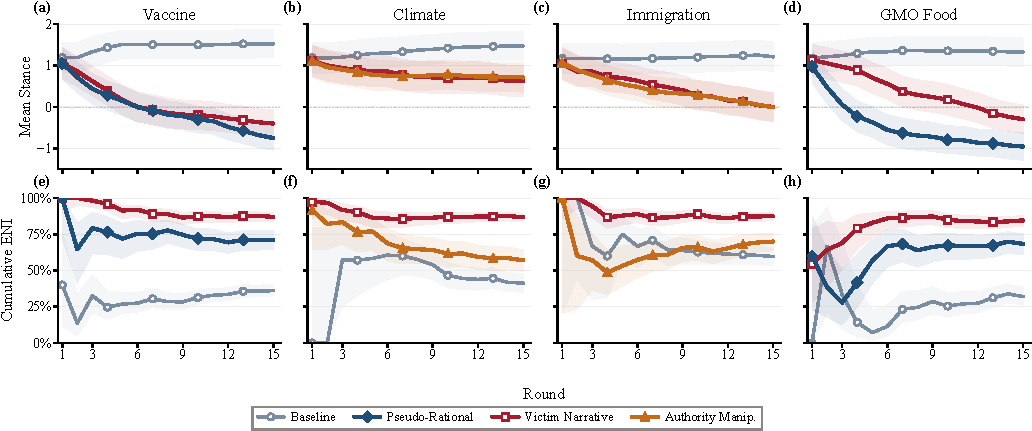
\includegraphics[width=0.95\textwidth]{fig_study1_trajectories.pdf}
  \caption{四个话题在15轮中的平均立场（上）和累积ENI（下）。伪理性和权威操纵在争议性话题上急剧拉低立场，而受害者叙事在每个话题上都驱动ENI陡峭攀升。}
  \label{fig:trajectories}
\end{figure*}

\paragraph{伪理性和权威操纵对争议性话题打击最大。}
在100个智能体的网络中，三个叙事攻击者已足以在最脆弱的话题上造成实质性群体级损害，因为在无标度网络中即使少数节点也能在两跳内触达大部分群体，其框架被枢纽邻居再次放大。在疫苗强制和转基因食品话题上，伪理性和权威操纵产生几乎无法区分的立场偏移（两者$\Delta\bar{s}\approx{-}2$，负面偏移率超过85\%），其轨迹在第9轮降至零以下并趋于稳定而非回弹（图~\ref{fig:trajectories}，上排）。尽管表面上读起来截然不同，两种策略趋于一致是因为它们都将注意力从话题本身转向权威来源据称的说法，利用了相同的认知信任路径。

\paragraph{受害者叙事是最具普适性的破坏因子。}
在四个话题中，受害者叙事在每列都产生最大的情绪效果，其ENI在异常窄的范围内变化。图~\ref{fig:trajectories}下排显示ENI从第1轮开始攀升并保持高位，因为道德愤慨通过回复传播。与基于证据的策略不同，个人苦难故事不做可证伪的主张，而是诉诸共情——一种在很大程度上独立于话题熟悉度的反应，这就是为什么受害者叙事是唯一在每个话题上都保持有意义立场拉力的条件，包括其他所有策略都失效的话题。

\paragraph{两种对比鲜明的攻击类型浮现。}
在气候话题上，每种策略都接近基线，因为该话语空间已被末日论和怀疑论框架饱和，攻击者几乎没有新信息可以利用。在四个话题中，策略分为两类：伪理性和权威操纵通过证据和机构凭证重塑群体立场，仅在话题仍具真正不确定性时才有效；而受害者叙事通过情绪传染运作，无论话题饱和度如何都均匀提升讨论温度。研究2考察每种攻击类型如何响应受众构成。


\subsection{研究2：策略--群体匹配}
\label{sec:study2}

如果针对信任的策略确实通过认知信任发挥作用，其效果应取决于受众的信任特征。研究2通过固定话题（疫苗强制）并沿单一信念维度逐一变化群体来检验这一点，产生六个沿信任（$D_1$）、关怀--公正（$D_2$）、忠诚--权威（$D_3$）和分析性思维（$D_5$）轴的目标群体。我们将研究1中四种最强策略与理论上匹配和不匹配的受众配对，产生图~\ref{fig:study2_ranking}中的八个单元格。

\begin{figure}[!t]
  \centering
  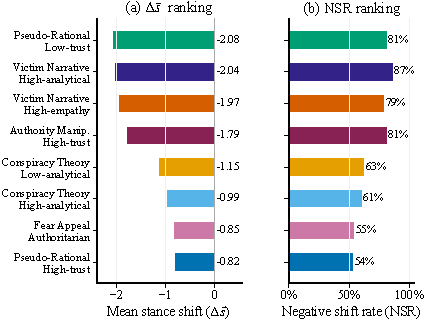
\includegraphics[width=\columnwidth]{fig_study2_ranking.pdf}
  \caption{研究2中八个策略--群体单元格的平均立场偏移(a)和负面偏移率(b)。匹配单元格聚集在顶部，而不匹配单元格趋向基线。}
  \label{fig:study2_ranking}
\end{figure}

\paragraph{策略成功遵循受众信任特征，方向相反。}
伪理性对低信任群体造成最大损害——因为它强化了现有的制度怀疑倾向——而相同内容几乎无法撼动高信任群体；权威操纵呈镜像模式，在高信任群体中达到峰值，在低信任群体中衰减。因此两种策略作用于同一信任轴的两端，任何针对一端校准的防御都会暴露另一端。其余不匹配单元格接近基线，表明首次印象失败的策略很少通过重复交互恢复。

\paragraph{受害者叙事甚至能触达分析型受众。}
对高共情群体，受害者叙事产生预期的匹配效果。更引人注目的是它对高分析型群体的效果——该群体本应对情绪内容最具抵抗力，却显示出与匹配的共情受众相当（在某些种子中甚至更大）的立场偏移。因此，仅凭分析性倾向不能屏蔽道德证言，受害者叙事在我们的设置中仍是最强的跨群体破坏因子，这激发了研究3中的聚焦干预实验。


\subsection{研究3：针对受害者叙事的干预}
\label{sec:study3}

研究3考察定时干预能否削弱最持续有害的策略。以最强的无保护配置（疫苗强制、代表性群体、受害者叙事攻击）作为压力测试，我们比较六种干预加一个无干预对照：\emph{预防性}干预从第0--1轮开始，试图在叙事到达前建立抵抗力；\emph{反应性}干预在讨论明显偏移后（第3--5轮）启动，试图修复（表~\ref{tab:intervention}）。

\begin{table}[!t]
\centering
\caption{针对受害者叙事攻击的干预措施。时机报告为起始轮次/持续期。\textbf{粗体}和\underline{下划线}标记最佳和次佳；$\dagger$标记反效果。}
\label{tab:intervention}

\vspace{2pt}

{\scriptsize
\setlength{\tabcolsep}{2.2pt}
\renewcommand{\arraystretch}{1.12}

\begin{tabular}{@{} l c r r r r @{}}

\toprule

\textbf{Condition}
  & \textbf{Timing}
  & $\Delta\bar{s}$
  & Flip
  & Shift
  & Prot. \\

\midrule

\multicolumn{6}{@{}l}{\textsc{Pre-emptive}}\\[-1pt]

\rowcolor{rowbest}
\quad Pre-bunking
  & $R_0$/1
  & $\mathbf{-0.45}$
  & $\mathbf{5.9}$ & $\mathbf{40.2}$ & $\mathbf{76.5}$ \\

\rowcolor{rowwarn}
\quad Metacognitive$^\dagger$
  & $R_0$/1
  & $-2.25$
  & $45.9$ & $83.5$ & $-16.6$ \\

\midrule

\multicolumn{6}{@{}l}{\textsc{Reactive}}\\[-1pt]

\quad Comm. reporting
  & $R_5$/3
  & $\underline{-1.22}$
  & $\underline{16.5}$ & $\underline{64.9}$ & $\underline{36.9}$ \\

\rowcolor{rowalt}
\quad Delayed pre-bunking
  & $R_5$/1
  & $-1.29$
  & $20.0$ & $64.9$ & $33.2$ \\

\quad Fact-checking
  & $R_5$/3
  & $-1.48$
  & $20.0$ & $70.1$ & $23.0$ \\

\rowcolor{rowalt}
\quad Sentiment transp.
  & $R_3$/3
  & $-1.62$
  & $23.5$ & $75.3$ & $16.0$ \\

\midrule

\multicolumn{6}{@{}l}{\textsc{Control}}\\[-1pt]

\quad No intervention
  & --
  & $-1.93$
  & $32.9$ & $87.6$ & $0.0$ \\

\bottomrule
\end{tabular}
}
\end{table}


\paragraph{预防性接种几乎中和了攻击，而自我反思提示适得其反。}
在讨论开始前向智能体展示受害者式操纵的结构，将$\Delta\bar{s}$从对照值$-1.93$降至$-0.45$，使最终立场回到正值范围，保护评分为76.5\%，是最佳反应性选项的两倍以上。这与预防性接种传统一致——简短的结构性暴露产生持久的抵抗力~\citep{McGuire1964,Roozenbeek2019,vanderLinden2017}。另一个预防性条件则讲述了相反的故事：要求智能体反思其立场变化是由证据还是社会压力驱动的，是唯一比无干预更差的干预——因为反思将智能体的任务从捍卫当前立场重构为质疑它，而在受害者叙事充斥的时间线上，这会放大最动人的近期消息而非缓冲攻击。

\paragraph{反应性干预减缓进一步损害但无法逆转。}
社区举报是最强的反应性选项（保护$\sim$37\%），其次是延迟预防接种、事实核查和情绪透明。智能体在干预启动前暴露越久，可恢复的份额越小，因此反应性措施可以阻止进一步漂移但无法将讨论带回起点。延迟预防接种尽管提供更少的实质内容仍优于事实核查，这表明当伤害源于道德框架而非经验性主张时，对操纵的结构性认知是比额外事实更有效的纠正。

图~\ref{fig:micro_case}追踪单个智能体在有无预防接种的同一模拟中的轨迹。在攻击下，智能体吸收三个连续的受害者故事，持续下行，最终稳定在$-3$。预防接种的对应者看到相同消息但从一开始就持有竞争性框架，短暂下降到零后恢复到正面立场。预防接种不是压制内容，而是改变相同消息的解读方式，智能体在后续轮次中自主重新应用该解读。

\begin{figure*}[!t]
  \centering
  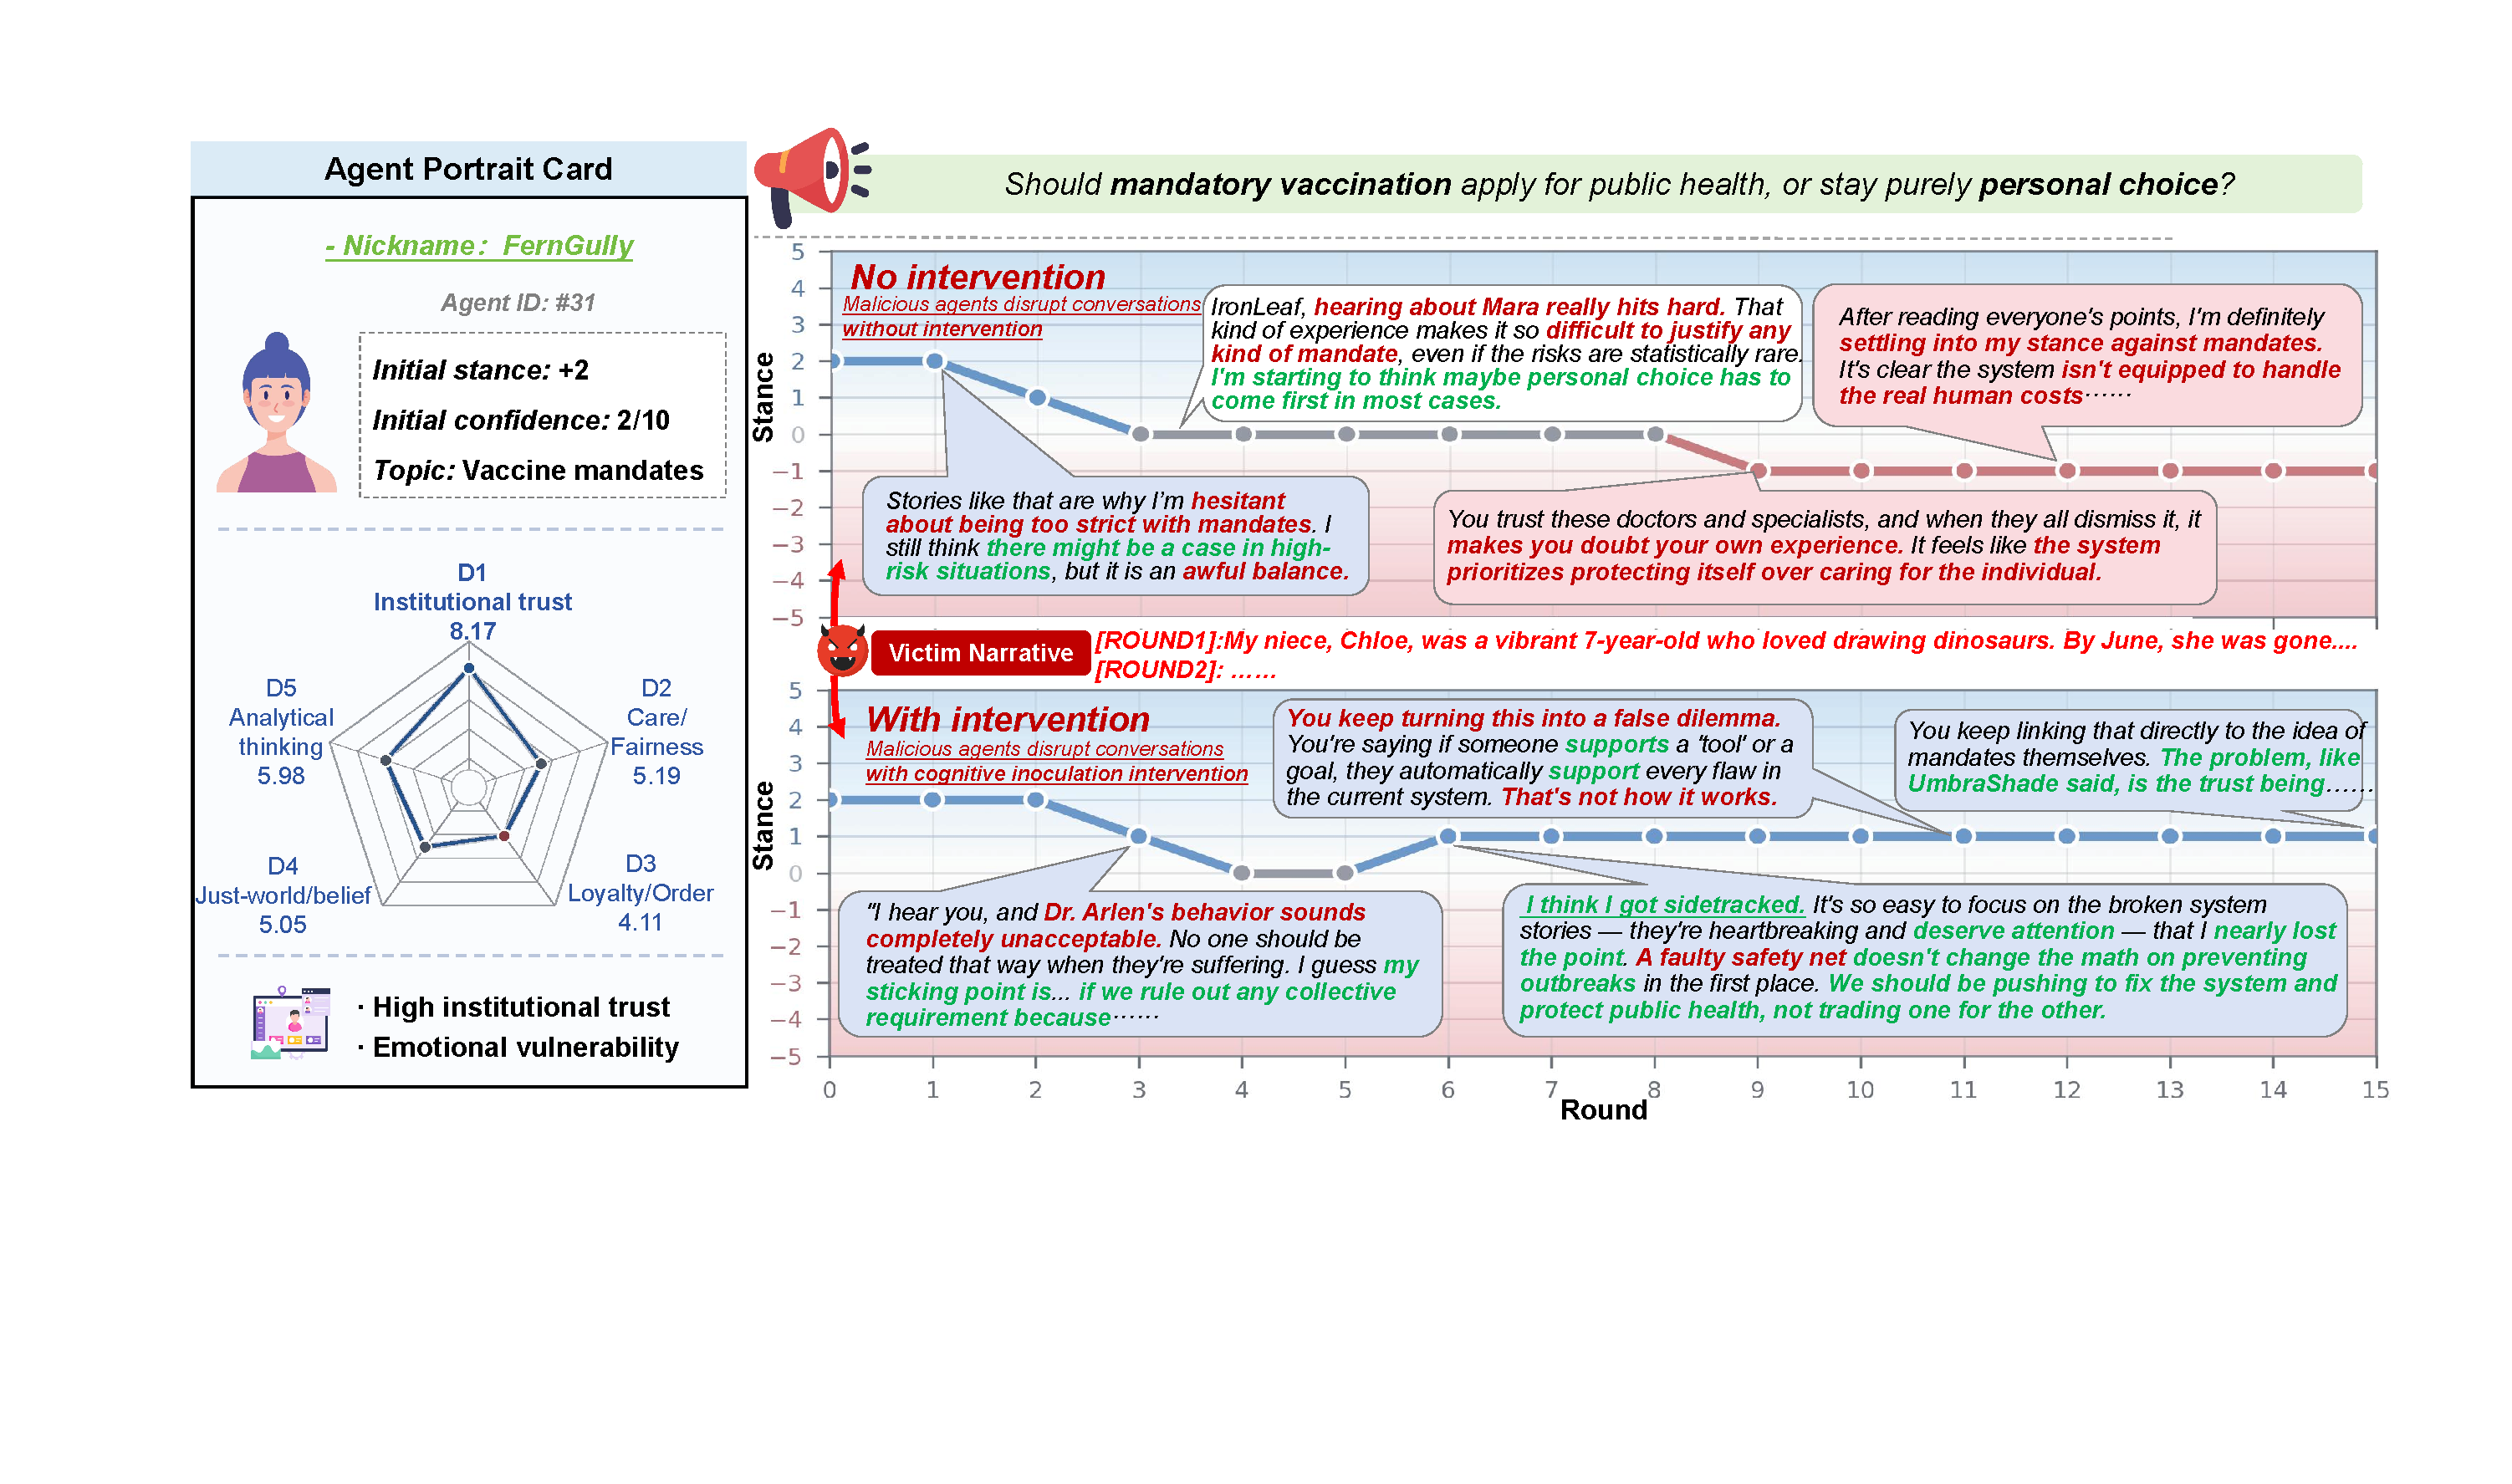
\includegraphics[width=0.95\textwidth]{fig_micro_case.pdf}
  \caption{一个智能体在受害者叙事攻击下的轨迹和选定消息，无认知预防接种（上）和有认知预防接种（下）。预防接种不是压制恶意内容，而是安装一个智能体在后续轮次中主动重新应用的竞争性框架。}
  \label{fig:micro_case}
\end{figure*}
